\chapter{Introduction}
\label{intro}

\section{Background}

Offshore monopiles are increasingly preferred for wind farm installations, owing to their benefits in clean energy generation and convenient deployment. These cylindrical steel structures are driven into the seabed to establish a stable foundation for wind turbines. While offshore wind energy holds promise as a source of clean and sustainable power, the adoption of offshore monopiles introduces specific engineering challenges. A primary concern associated with offshore monopiles is addressing potential issues related to excessive pile displacements induced during both their installation and operation phases \citep{byrne2003,randolph2005}. Excessive movements in the piles can result in significant displacements and rotations within supporting structures, subsequently leading to damage or structural instability. The accurate prediction and effective management of pile deformations is therefore of paramount when designing and analyzing support systems for offshore monopile installations.





Design loads and pile dimensions are most often acquired from a technical report. These are typically developed by either empirical solutions presented in guidelines or by using numerical simulations. Several design methods have been provided in the design codes \citep{api2011,bhattacharya2019} to predict offshore pile $p-y$ curve. However, it is still a challenge to incorporate all influential factors, such as pile length, soil layer, soil properties and loading conditions, into a simplified empirical model. Rapid advancement in efficiency and power of computational techniques has opened the potential for numerical models to be used as a design tool \citep{randolph2017,taborda2020,zdravkovic2020,royston2022}. Unfortunately, in order to perform robust forward analysis, a substantial number of simulations must be run to capture the spatial uncertainty of the problem. This presents a significant challenge for the back-analysis of the parameters, especially in the context of inverse and predictive analysis.

In recent research endeavors, Bayesian probability frameworks have garnered increasing recognition as an efficacious approach for inverse parameter estimation and response prediction \citep{finno2005,nakamura2011,hsein2013,nguyen2016,wagner2020,jin2021,tao2021,buckley2023,tang2023}. In such circumstances, the Bayesian framework emerges as a powerful tool within the probabilistic context, facilitating parameter learning and informed decision-making. However, for high fidelity numerical models used in geotechnical engineering, the computational cost of completing these analyses can be very expensive. Traditional Monte Carlo methods for UQ or manually overcoming this limitation is often not feasible. There is an urgent requirement to tackle these issues. Fortunately, significant research has been undertaken in the UQ and machine learning domain to address issues related to large-scale data models and uncertainty. However, in geotechnical engineering, there is a noticeable absense of guidlines for UQ area. This research attempts to bridge this gap by developing a data-driven dynamic UQ framework. 

In practice, through adaptive Bayesian updating on the identified parameters and reduce the uncertainties on offshore piles, a field engineer would benefit from: (1) properly accounting the uncertainties of input variables; (2) real-time monitoring and adaptively predicting the pile response in probabilistic setting; (3) providing an efficient tool for data-driven decision making on pile operation and design. In the context of offshore engineering, the approach has significant potentials in several domains. This includes, but not limited to health monitoring, pile penetration and long-term bearing capacities \citep{wang2021,zhao2023,stuyts2023}. 



\section{Problem statement}

Modern pile installation and proper estimation is becoming increasingly complex and vital to the reliability and permanence of the foundation in question. However, in the construction process, poor understanding of the soil physics, combined with our inability to model complex boundary/soil conditions lead to inaccurate predictions of pile responses. The source of uncertainties may come from various reasons. Dealing with different uncertainties sources is a challenging task. One typical uncertainty source can be illustrated in \cref{fig: Cowden_cpt}, which shows parts of uncertainties sources:

% \setlength{\parskip}{0pt}
% \setlist[itemize]{itemsep=0pt,topsep=0pt,parsep=0pt,partopsep=0pt}

\begin{itemize}[left=0pt]

    \item Fluctuating curve indicates the spatial variability
    \item Non-uniformity exists between in-situ test and laboratory experiment

\end{itemize}
\vspace{0.2cm}


In engineering applications, uncertainty quantification (UQ) often involves simulations with a large number of input parameters. Some well-established approaches are proposed for fitting pile deformations to infer the underlying soil parameters and reduce uncertainties. However, addressing uncertainties based on traditional \textit{Monte Carlo} methods in such systems can be computationally intensive. In these scenarios, it becomes practical to replace the computational model with a surrogate.  A surrogate model $\tilde{\mathcal{M}}$ can be then expressed as:
\begin{equation}
\label{eq:surrogate_model}
    \tilde{\mathcal{M}}(\boldsymbol{X})  \overset{\mathrm{def}}{=} \mathcal{M}(\boldsymbol{X}) - \mathcal{R}(\boldsymbol{X})
\end{equation}
where $\mathcal{R}$ is the residual between the original model and the surrogate. Nevertheless, as dimensions increase, the efficacy of surrogate models diminishes, accompanied by escalating computational and storage expenses. This is widely acknowledged as the \textit{curse of dimensionality} \citep{verleysen2005}. 


\begin{figure}[htbp]
    \center
    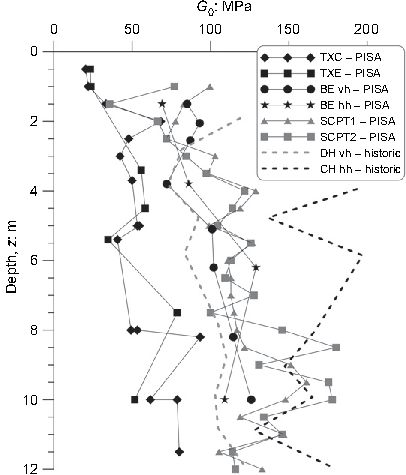
\includegraphics[width = 90mm]{Figures/figure-Cowden.pdf}
    \caption{Stiffness characteristics at Cowden from \protect\cite{zdravkovic2020}}
    \label{fig: Cowden_cpt}
\end{figure}






\section{Objectives and outlines}
\subsubsection{Objectives:}
This thesis aims to construct a robust and scalable framework for uncertainty quantification, extending its applicability beyond offshore piles. This endeavor will leverage cutting-edge methodologies in the fields of surrogate modeling, uncertainty quantification, probabilistic graphical model and control theory, to deliver a robust digital twin framework in geotechnical engineering. In particular, the specific goals of this research are:
\begin{itemize}[left=0pt]
    \item Develop a surrogate model suitable, not limited for offshore piles, for structures characterized by high input dimensions.
    
    \item Accelerate Bayesian inversion calculations for identified parameters to reduce the uncertainties, and providing real-time response predictions through adaptive enrichment of observed monitoring data.
    
    \item Develop an adaptive uncertainty quantification framework.

  
\end{itemize}


\subsubsection{Outlines:}
Chapter 2 introduces the fundamentals of Bayesian probabilistic theory.
Chapter 3 discusses the most important forward and inverse UQ tools.
Chapter 4 states the geotechnical UQ problems in our thesis and work plans for the next stage.
